\documentclass[
  a4paper,            % DIN A4
  DIV=10,             % Schriftgröße und Satzspiegel
  oneside,            % einseitiger Druck
  BCOR=5mm,           % Bindungskorrektur
  parskip=half,       % Halber Abstand zwischen Absätzen
  numbers=noenddot,   % Kein Punkt hinter Kapitelnummern
  bibtotoc,           % Literaturverzeichnis im Inhaltsverzeichnis
  listof=totoc,       % Abbildungs- und Tabellenverzeichnis im Inhaltsverzeichnis
  table
]{scrreprt}
\usepackage{../style/thesisstyle}

\makeglossaries           % create all glossary entries (remember: run makeglossaries manually)
\loadglsentries{thesisglossaries.tex}  % load acronym, symbol and glossary entries

\sisetup{locale = DE}     % siunitx locale setup
%\DeclareSIUnit \fps{fps}  % a custom unit (usage: \SI{24}{\fps})

\begin{document}
% !TEX root = ../thesis.tex
%
% configurations
%

% English Language support
% -> uncomment if needed
% Beta!
%\fullenglish{yes}
\fullenglish{no}

% text field
%-> replace supervisor names with correct ones
\firstSupervisor{Prof. Dr. Philipp Jenke}
\secondSupervisor{Prof. Dr. Peer Stelldinger}

% text field
%-> replace title with your thesis title
\thesisTitle{Beispiel-basierte inverse prozedurale Generierung für zweidimensionale Szenen}
\thesisTitleEN{Example-based inverse procedural generation for two-dimensional scenes}

% text field
%-> replace the key words with your own key words
\keywordsDE{TODO SCHLÜSSELWÖRTER}
\keywordsEN{TODO KEYWORDS}

% text field
%-> replace the text with a description of the thesis
\abstractDE{TODO ZUSAMMENFASSUNG}
\abstractEN{TODO ABSTRACT}

% text field
%-> replace john with your name
\thesisAuthor{Benjamin Schröder}

% text field
%-> enter the submission date
\submissionDate{11. Juli 2024}

% switch - uncomment only one
%-> uncomment NDA or public
%\NDA{yes}
\NDA{no}

% switch - uncomment only one
%-> uncomment old standard cover or cover Corporate Design 2017
\Cover{CD2017}
%\Cover{CD2017NoLogo}
%\Cover{Std2018}
%\Cover{Std2018_green} 			% with green bar

% switch - uncomment only one
%-> uncomment to show list of figures or not
\ListOfFigures{yes}
%\ListOfFigures{no}

% switch - uncomment only one
%-> uncomment to show list of tables or not
\ListOfTables{yes}
%\ListOfTables{no}

% switch - uncomment only one
%-> uncomment to show list of accronyms or not
\ListOfAccronyms{yes}
%\ListOfAccronyms{no}

% switch - uncomment only one
%-> uncomment to show list of symbols or not
\ListOfSymbols{yes}
%\ListOfSymbols{no}

% switch - uncomment only one
%-> uncomment to show list of glossary entries or not
\Glossary{yes}
%\Glossary{no}

% switch - uncomment only one
%-> uncomment the study course you are in
%\studycourse{ITS}
%\studycourse{TI}
\studycourse{AI}
%\studycourse{WI}
%\studycourse{EI}
%\studycourse{REE}
%\studycourse{BMP}		
%\studycourse{BMP-hp}	 % Internship Report in M&P
%\studycourse{BMT}
%\studycourse{BMT-st}    % Study / home assignment in BMT
%\studycourse{BMT-hp}    % Internship Report in BMT
%\studycourse{MI}
%\studycourse{MIK}
%\studycourse{MA}

\def\imgHeight{100pt}
\def\imgWidth{420pt}
    % load all settings

\hyphenation{Ba-che-lor-the-sis Mas-ter-the-sis}

% Cover page here, no page number
\ICoverPage

% PDF Metadata
% !TEX root = ../thesis.tex
%
% PDF Metadata integration
% @author Thomas Lehmann
%

% PDF Metadata
\hypersetup{
pdftitle={\IthesisTitle},
pdfauthor={\IthesisAuthor},
pdfkeywords={\IkeyWordsEN}
}

% Titlepage is page one even if the number is not shown.
\pagenumbering{roman}
% Title page here
% !TEX root = ../thesis.tex
%
% title page
% @author Thomas Lehmann
% Hints for title page and page numbering: https://en.wikipedia.org/wiki/Title_page
%
\title{\IthesisTitle}   % set latex default title to be used by hyperref in pdf
\author{\IthesisAuthor} % set latex default author to be used by hyperref in pdf

\newpage
\thispagestyle{empty}
{\fontfamily{phv}\selectfont
  \hfuzz=20pt       % suppress warnings due to extension onto page margins

  % Author of thesis
  \vspace*{1cm}
  \begin{minipage}[b]{\textwidth}
    \fontsize{14pt}{20pt}
    \selectfont
    \begin{center}
      \IthesisAuthor
    \end{center}
  \end{minipage}

  % Title of thesis
  \vspace{1.5cm}
  \begin{minipage}[b][0cm][t]{\textwidth}
    \fontsize{18pt}{20pt}
    \selectfont
    \begin{center}
      \IthesisTitle
    \end{center}
  \end{minipage}

  % Important information
  \begin{textblock*}{\textwidth}(40mm,210mm)
    \begin{minipage}[b]{\textwidth}
      \hbadness=10001    % suppress underfull warning due to short text
      \fontfamily{cmr}\selectfont
      \fontsize{12pt}{14pt}
      \selectfont
      \ifdefined\ILanguageEN
        \IthesisKindEN ~submitted for examination in \IthesisExaminationEN \\
        in the study course \textit{\IstudyCourseName} \\
        at the \IthesisDepartmentFullEN \\
        at the \IthesisFacultyFullEN \\
        at University of Applied Science Hamburg\\

        Supervisor: \IfirstSv \\
        \ifdefined\IisTermPaper
          % left blank
        \else
          \ifdefined\IisInternshipReport
	  Supervised: \IsecondSv\\
          \else
        Supervisor: \IsecondSv \\
          \fi\fi
        
        Submitted on: \ISubDate \\
      \else
      	\ifdefined\IisInternshipReport
        \IthesisKindDE ~eingereicht im Rahmen des \IthesisExaminationDE \\	
	\else
        \IthesisKindDE ~eingereicht im Rahmen der \IthesisExaminationDE \\
        \fi
	im Studiengang \textit{\IstudyCourseName} \\
        am \IthesisDepartmentFull \\
        der \IthesisFacultyFull \\
        der Hochschule für Angewandte Wissenschaften Hamburg\\

        Betreuender Prüfer: \IfirstSv \\
        \ifdefined\IisTermPaper
          % left blank
        \else
          \ifdefined\IisInternshipReport
        betriebliche Betreuung: \IsecondSv \\							
	  \else
        Zweitgutachter: \IsecondSv \\
        \fi\fi

        Eingereicht am: \ISubDate \\
      \fi
    \end{minipage}
  \end{textblock*}
}


% Abstract page here
% !TEX root = ../thesis.tex
%
% abstract page
% @author Thomas Lehmann
%
\newpage
\thispagestyle{plain}
\clearpage
\hfuzz=12pt       % suppress warnings due to extenstion onto page margins

\textbf{\IthesisAuthor}

\vspace{0.3cm}
\textbf{Thema der Arbeit}

\IthesisTitle

\vspace{0.3cm}
\textbf{Stichworte}

\IkeyWordsDE

\vspace{0.3cm}
\textbf{Kurzzusammenfassung}

\begin{minipage}{\textwidth}
\IabstractDE
\end{minipage}

\vspace{1.0cm}
\textbf{\IthesisAuthor}

\vspace{0.3cm}
\textbf{Title of Thesis}

\IthesisTitleEN

\vspace{0.3cm}
\textbf{Keywords}

\begin{minipage}{\textwidth}
\IkeyWordsEN
\end{minipage}

\vspace{0.3cm}
\textbf{Abstract}

\IabstractEN


% Table of contents here
\tableofcontents

% List of figures here
\IListOfFigures

% List of tables here
\IListOfTables

% List of accronyms here
\IListOfAccronyms

% List of symbols here
\IListOfSymbols

% Uncomment if list of source code is needed (rarely).
%\lstlistoflistings  % requires package listings, needs to uncommenting of usepackage

% path to the chapters folder is set to find the images used there
\graphicspath{ {./chapters/} }

% Chapters
\clearpage
\pagenumbering{arabic}
% @author Benjamin Schröder
%
\chapter{Einleitung}

\section{Motivation}
% In diesem Abschnitt wird erklärt, wieso die prozedurale Generierung überhaupt so ein wichtiges Thema ist.
% Es wird geklärt, wer davon Gebrauch macht, und wieso es für den entsprechenden Anwender Sinn macht. Dazu zählt
% zum Einen das Einsparen von Ressourcen, aber auch das Umsetzen von Spielkonzepten, die durch die hier vorgestellten
% Verfahren erst möglich werden.
Die Erstellung von fiktiven Welten spielt eine große Rolle in vielen Videospielen, Filmen, Virtual Reality Umgebungen
und weiteren Bereichen der Simulation. Hierfür wird eine Vielzahl an verschiedenen Objekten und Strukturen benötigt, um
ein nicht-repetitives und immersives Erlebnis für den Endnutzer zu schaffen. All dies manuell anzufertigen, stellt vor
allem kleinere Indie-Entwicklerstudios vor eine große Herausforderung und kann die Entwicklungszeit signifikant in die
Länge ziehen. Aber auch in größeren Teams mit einer Vielzahl von Designern nimmt die Erstellung von realistischen Welten einen
Großteil der Entwicklungszeit in Anspruch und kann viele Monate dauern. \cite{10_freiknecht} Hier kann an einigen Stellen
nachgeholfen werden, indem man das Erstellen von Inhalten automatisiert. Entsprechende Prozesse lassen sich dem Bereich
der prozeduralen Generierung zuordnen.

Mithilfe von verschiedensten Verfahren können so z.B. einzelne Dungeons oder sogar ganze Welten und darin enthaltene Gebilde
automatisch erzeugt werden. Diese können eine Grundstruktur für ein komplexeres Design bilden, bei dem die Entwickler dann nur noch
kleinere Details per Hand abändern oder hinzufügen müssen. \cite{10_freiknecht} Andererseits existieren auch viele Videospiele,
wie z.B. Minecraft\footnote{\url{https://www.minecraft.net/} [Letzter Zugriff am 01.07.2024]} oder Terraria\footnote{
\url{https://terraria.org/} [Letzter Zugriff am 01.07.2024]}, die auf prozeduraler
Generierung aufbauen, um ihr Spielkonzept umzusetzen. Konkret wird einem neuen Spieler hier eine komplett neue und einzigartige,
aber dennoch logisch zusammenhängende Welt generiert; dies vollautomatisch und ohne zusätzlichen Aufwand für die Entwickler. Jeder
Spieler bekommt so eine einzigartie Erfahrung geboten und kann das Spiel außerdem gewissermaßen unbegrenzt oft durchspielen, ohne
dass es zu repetitiv wird. So etwas wäre ohne Automatisierung gar nicht erst umsetzbar.

\section{Problemstellung}
% Hier wird dann darauf aufmerksam gemacht, dass es bei diesen Verfahren viele Limitationen gibt. Bei vielen Verfahren
% ist es nötig, manuell Regeln für den Algorithmus zu erstellen, sodass dieser überhaupt arbeiten kann. Dies setzt wiederum
% einiges an Kenntnissen voraus und ist somit nicht für jeden zugänglich. Außerdem werden weitere Probleme aufgezeigt.

% Alte Formulierung:
% Es gibt viele bekannte Verfahren, welche solche Ergebnisse unter der Verwendung von u.a. zellulären Automaten, generativen
% Grammatiken oder Constraint-basierten Graphen erzielen können. \cite{5_van_der_linden_et_al} Ein Großteil dieser Verfahren erfordert jedoch
% menschliches Eingreifen in einigen der Teilschritte. So z.B. muss beim Verwenden einer generativen Grammatik meist bereits eine Menge
% an Produktionsregeln durch einen Menschen vorgegeben werden, bevor die automatische Generierung überhaupt beginnen kann. Das Erstellen
% solcher Regeln ist mit viel Arbeit und Trial-and-Error verbunden und kann ohne ein ausgeprägtes Verständnis des angewandten Verfahrens
% sehr schwierig werden. Dadurch kommt es für viele Designer letztendlich doch nicht in Frage. Auch gibt es Szenarien, in denen die Generierung
% von Inhalten durch den Endnutzer beeinflusst werden kann, so z.B. in Spielen, in denen der Spieler dynamisch mit dem Terrain und anderen
% Strukturen interagieren kann. In einem solchen Fall kann der Entwickler keinen direkten Einfluss auf den Generierungsprozess nehmen und alles
% muss voll automatisiert sein. \cite{14_carli_et_al} Hier setzt diese Arbeit an und untersucht Möglichkeiten zur vollständigen Automatisierung
% solcher Verfahren.

Es gibt viele bekannte Verfahren, welche solche Ergebnisse unter der Verwendung von u.a. generativen
Grammatiken oder Constraint-basierten Graphen erzielen können. \cite{5_van_der_linden_et_al} Ein Großteil dieser Verfahren erfordert jedoch
menschliches Eingreifen in einige der Teilschritte, was in einigen Szenarien zu einem Problem werden kann. Hängt die Generierung von
Inhalten eines Produkts z.B. von Entscheidungen des Endnutzers ab (z.B. in Spielen, in denen der Spieler dynamisch mit
dem Terrain und anderen Strukturen interagiert), so kann der Entwickler keinen direkten Einfluss auf den Generierungsprozess
nehmen und alles muss voll automatisiert sein. \cite{14_carli_et_al} Auch in Projekten, in denen dies nicht der Fall ist und der gesamte Inhalt
im Voraus erstellt wird, kann das Voraussetzen von menschlicher Intervenierung als Teil des Prozesses zu einem Problem werden.
Ein Beispiel hierfür wären Verfahren, die eine generative Grammatik nutzen und voraussetzen, dass dafür zunächst eine Menge an Regeln
durch einen Menschen vorgegeben wird, bevor die automatische Generierung überhaupt beginnen kann (z.B. \cite{33_adams}\footnote{
\url{https://citeseerx.ist.psu.edu/document?repid=rep1&type=pdf&doi=25020f8d955aee07b7dd49a3ec23b1f2a8cf1d06} [Letzter Zugriff am 01.07.2024]}).
Das Erstellen solcher Regeln ist mit viel Arbeit verbunden und kann ohne ein ausgeprägtes Verständnis des angewandten Verfahrens sehr
schwierig werden, wodurch der Einsatz eines solchen Verfahrens für viele Designer letztendlich doch nicht in Frage kommen wird. Hier
setzt diese Arbeit an und untersucht Möglichkeiten zur Automatisierung des Erstellens solcher Regeln.

\section{Ziele und Vorgehen}
% Aus den aufgezeigten Problemen ergibt sich nun der Sinn dieser Arbeit. Inverse Verfahren beheben die oben genannten Probleme
% und sollen deswegen genauer untersucht werden. Es werden verschiedene Verfahren analysiert und miteinander verglichen.
% Anschließend wird ein entsprechendes und vielversprechendes Verfahren im Detail untersucht, theoretisch erläutert und
% dann prototypisch implementiert.
Spezifisch soll versucht werden, Muster in Beispielstrukturen zu identifizieren. Aus diesen Mustern sollen dann Regeln zum Zusammensetzen
von Strukturen mit ähnlichen Eigenschaften abgeleitet werden. Gelingt dies, so muss ein Designer lediglich ein einziges Beispielmodell erstellen und
kann damit eine kreative Vision vorgeben. Alle weiteren Schritte zum Ableiten von Variationen dieses Inputs laufen anschließend automatisch ab.
Dies nennen wir \textit{inverse} prozedurale Generierung,
da der Prozess mit einem soweit fertigen Modell beginnt und daraus dann die Regeln ableitet, statt wie in den klassischen Verfahren zuerst mit
der Erstellung der Regeln zu beginnen. Die Erstellung eines Beispielmodells erfordert zwar nach wie vor die Arbeit eines Designers, anschließend
ist aber kein menschliches Eingreifen mehr nötig und das eigentliche Verfahren läuft vollautomatisch ab.

Es gibt bereits verschiedene Verfahren, die einen solchen Ansatz verfolgen. Diese sind u.a. der Gitter-basierte Wave Function
Collapse Algorithmus von Maxim Gumin \cite{45_gumin} oder die nach Symmetrien suchende inverse prozedurale Modellierung von Bokeloh
et al. \cite{3_bokeloh_et_al}.

Im Rahmen dieser Arbeit werden entsprechende Verfahren grob analysiert, deren Probleme aufgezeigt und anschließend ein neuer Ansatz vorgestellt,
welcher die vorhandenen Probleme minimieren soll. Das Endergebnis der Arbeit soll dann sein, dass die Funktionsweise des neuen Konzepts
ausführlich und verständlich dargestellt, und dieses anschließend prototypisch implementiert wird. Wir begrenzen uns dabei auf die Generierung von
Strukturen im zweidimensionalen Raum. Der gleiche Ansatz kann auch auf den dreidimensionalen Raum erweitert werden, um so vielseitiger einsetzbar zu
sein, jedoch reicht die vereinfachte Betrachtung zum Darstellen aller fundamentalen Konzepte.
% @author Benjamin Schröder
%
% Quellen: 5, 9, 10, 14, 15, 16, 17, 18, 19, 24, 25
%
% 5:
%   - Definition von PCG
%   - Vorstellen von einigen Verfahren
%
% 9:
%   - Definition von PCG durch Abgrenzung von anderen Verfahren
%
% 10:
%   - Geschichte und Verwendung von PCG
%   - Vorstellen einiger Verfahren
%
% 14:
%   - Vorstellen einiger Verfahren
%   - Unterscheidung zwischen assisted/non-assisted
%
% 15: The Death of the Level Designer
%   - kurze Definition von PCG
%   - Übersicht zu verschiedenen Anwendungsmöglichkeiten von PCG
%
% 16: An Image Synthesizer
%   - Perlin Noise
%
% 17: A Survey of Procedural Noise Functions
%   - Verwendung von Noise für PCG
%
% 18: Improving Noise
%   - Verbesserung von Perlin Noise
%
% 19: Fractals and the Geometry of Nature
%   - Fraktale (Mandelbrot)
%
% 24: A Very Short History of Dynamic and Procedural Content Generation
%   - Geschichte von PCG
%
% 25: Procedural Content Generation for Games: A Survey
%   - Klassifikation verschiedener Arten von PCG
%
% Weitere Links:
%   - https://en.wikipedia.org/wiki/Procedural_generation
%   Perlin Noise:
%   - https://mzucker.github.io/html/perlin-noise-math-faq.html#whatsnoise
%   - https://adrianb.io/2014/08/09/perlinnoise.html
%   - https://mrl.cs.nyu.edu/~perlin/doc/oscar.html
%   Simplex Noise:
%   - https://thebookofshaders.com/11/?lan=de

\chapter{Grundlagen}
Als Grundlage für das Verständnis des weiteren Inhalts dieser Arbeit machen wir zunächst einen kurzen Abstecher in den
Bereich der prozeduralen Generierung allgemein. Wir stellen klar, was unter diesem Begriff zu verstehen ist und widmen
uns außerdem kurz der zugrundeliegenden Geschichte. Dabei werden wir einige fundamentale Errungenschaften und Verfahren
betrachten, die den Weg zum aktuellen Forschungsstand geprägt haben.

\section{Prozedurale Generierung}
Prozedurale Generierung, oder auch \gls{ac:pcg}, beschreibt eine Menge von Verfahren zum algorithmischen Erstellen von
Inhalten (``Content''). Dabei handelt es sich meist um Inhalte in Form von Texturen oder verschiedenen Gebilden im Kontext
von Videospielen und anderen Simulationen, wie z.B. Landschaften, Flüsse, Straßennetze, Städte oder Höhlenstrukturen.
\cite{14_carli_et_al} Auch Musik kann durch solche Verfahren generiert werden. \cite{28_ramanto_maulidevi}

Diese Definition ist absichtlich etwas allgemeiner gehalten, da das Aufstellen einer spezifischeren Definition nicht
besonders trivial ist. Das Konzept von \gls{ac:pcg} wurde bereits aus vielen veschiedenen Blickwinkeln beleuchtet und
ist für verschiedene Personen von unterschiedlicher Bedeutung. So hat z.B. ein Game Designer eine etwas andere Perspektive
als ein Wissenschaftler, der sich lediglich in der Theorie mit der Thematik beschäftigt. \cite{9_togelius_et_al}
Verschiedene Definitionen unterscheiden sich in Bezug auf Zufälligkeit, die Bedeutung von ``Content'', oder darin, ob und
in welchem Umfang menschliche Intervenierung eine Rolle in einem Verfahren spielen darf. Smelik et al. definieren ``Content''
als jegliche Art von automatisch generierten Inhalten, welche irgendwie anhand von einer begrenzten Menge an Nutzer-definierten
Parametern erzeugt werden können. \cite{26_smelik_et_al} Timothy Roden und Ian Parberry beschreiben entsprechende Verfahren zur
Erzeugung dieser Inhalte als \textit{Vermehrungsalgorithmen} (``amplification algorithms''), da diese eine kleinere Menge
von Inputparametern entgegennehmen und diese in eine größere Menge an Outputdaten transformieren. \cite{27_roden_parberry}
Togelius et al. \cite{9_togelius_et_al} versuchen den Bereich genauer abzugrenzen, indem sie anhand von Gegenbeispielen
aufzeigen, was \textit{nicht} als \gls{ac:pcg} bezeichnet werden sollte. So zählt für Togelius et al. z.B. das Erstellen von
Inhalten eines Videospiels mittels Level-Editor in keinem Fall als \gls{ac:pcg}, auch wenn dabei das Spiel indirekt durch z.B.
automatisches Hinzufügen oder Anpassen von Strukturen beeinflusst wird. Generell wird sich in der Arbeit
von Togelius et al. \cite{9_togelius_et_al} ausführlich mit dem Problem der Definition von \gls{ac:pcg} befasst, weshalb
dies hier nun nicht weiter thematisiert werden soll. Die oben genannte grobe Erklärung fasst die Kernaussage der verschiedenen
Definitionen weitesgehend zusammen und sollte für unsere Zwecke ausreichen.

\section{Geschichte von PCG}

\input{chapters/3_stand_der_technik}
% @author Benjamin Schröder
%
% Konzepte:
% - Splicing
% - Reduzierbarkeit (reducible graphs)
% - Irreducible Graphs (alle Graphen sind entweder reduzierbar oder unvollständig)

\chapter{Theorie}
Im Folgenden werden die theoretischen Konzepte hinter dem praktischen Teil der Arbeit betrachtet. Das implementierte Verfahren wird
Schritt für Schritt vorgestellt und im Detail erläutert. Die vorgestellten Konzepte beruhen auf den Erkenntnissen von Paul Merrell
in seiner Arbeit aus dem Jahr 2023 \cite{1_merrell}.

\section{Überblick}

\begin{figure}[t]
    \centering
    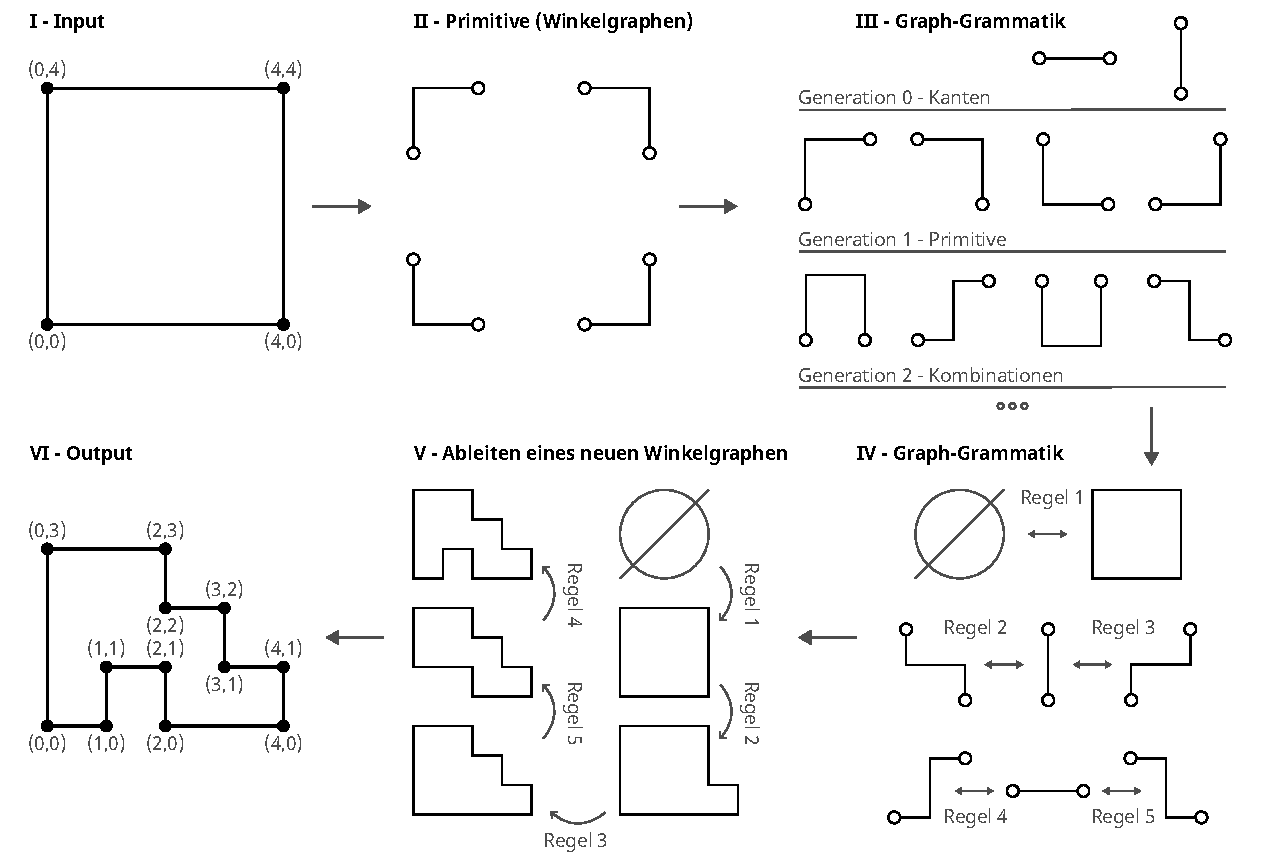
\includegraphics[width=\imgWidth]{images/overview.pdf}
    \caption{Überblick zum Ablauf des Verfahrens.}
    \label{fig:overview}
\end{figure}

Bevor es um die Einzelheiten und spezifischen Konzepte geht, wird zunächst ein grober Überblick zum Ablauf des umgesetzten
Verfahrens geliefert. Das Ganze beginnt mit einer polygonalen Inputstruktur, d.h. einem Gebilde bestehend aus einem oder mehreren Polygonen
(siehe Abbildung \ref{fig:overview}-I).
Diese Inputstruktur wird anschließend umgewandelt in einen Graphen, in welchem die konkrete Geometrie des Inputs keine Rolle
mehr spielt und sich auf die für das Verfahren wichtigen Eigenschaften des Inputs konzentriert werden kann.

Im nächsten Schritt wird der erstellte Graph nun in seine kleinstmöglichen Einzelteile zerlegt. Dazu werden alle Kanten in zwei Halbkanten
aufgeteilt. Das Ergebnis sind viele Teilgraphen, welche jeweils nur noch aus einem Knoten und einigen Halbkanten bestehen.
Einen solchen Teilgraphen nennen wir \textit{Primitiv}. Diese Primitive werden dann Schritt für Schritt in allen möglichen Kombinationen
zusammengeklebt, was zum Entstehen einer Hierarchie an immer komplexer werdenden Graphen führt (siehe Abbildungen \ref{fig:overview}-II und
\ref{fig:overview}-III).

Beim Aufbau der Hierarchie werden die neu entstehenden Graphen auf bestimmte
Eigenschaften überprüft, die es uns erlauben, daraus Regeln für eine Graph-Grammatik abzuleiten (siehe Abbildung \ref{fig:overview}-IV).
Das einfachste Beispiel hierfür sind
vollständige Graphen, also Graphen, die nur noch aus in sich geschlossenen Kreisen bestehen und keine Halbkanten mehr besitzen. Aus diesen lässt
sich eine sogennante Startregel ableiten, welche den leeren Graphen mit dem gefundenen vollständigen Graphen ersetzt. Das Finden von weiteren
Regeln ist deutlich komplizierter und wird später im Detail erläutert.

Sobald man nun eine Menge von Regeln für die Graph-Grammatik gefunden hat, kann man diese verwenden um verschiedenste zum Inputgraphen
ähnliche Graphen abzuleiten, indem zufällig verschiedene Regeln nach und nach angewendet werden (siehe Abbildung \ref{fig:overview}-V).
Für einen solchen Graphen müssen dann noch konkrete Knotenpositionen und Kantenlängen bestimmt werden, sodass dieser wieder als Struktur
aus Polygonen dargestellt werden kann (siehe Abbildung \ref{fig:overview}-VI).

\section{Grundlagen}
\subsection{Input}
Der Algorithmus kann mit beliebigen polygonalen Strukturen als Input arbeiten. Dies können einfache Rechtecke oder aber auch komplizierte Gebilde
aus verschiedenen Häusern oder ähnlichem sein. Wichtig ist lediglich, dass der Input als Sammlung von Polygonen beschrieben werden kann, welche
wiederum als Sammlung von Punkten und Kanten beschrieben werden können.
So sind z.B. Kreise oder andere Strukturen mit Rundungen kein valider Input und können wenn dann nur durch komplexe Polygone angenähert werden.
Die einzelnen Polygone können außerdem mit Farben versehen werden, um verschiedene Arten von abgegrenzte Bereichen im Input zu markieren.

\subsection{Der Winkelgraph}
Zur Verarbeitung des Inputs wird dieser in einen sogenannten Winkelgraphen umgewandelt, in welchem die spezifischen Positionen der Knoten
keine Rolle spielen. Stattdessen wird nur abgebildet, welche Knoten es überhaupt gibt, welche der Knoten durch Kanten miteinander verbunden
sind, und in welchem Winkel diese Kanten verlaufen.
Die Kanten im Graphen werden mit einem entsprechenden Label versehen, welches neben den Start- und Endknoten ebenfalls Informationen zum
daraus ableitbaren Tangentenwinkel, sowie zu den Farben der links und rechts anliegenden Polygone enthält. Ein Kantenlabel besitzt die Form
\(\tilde{k} = (l,r,\theta)\), wobei \(\tilde{k}\) die Bezeichnung der Kante, \(l\) und \(r\) die Farben der anliegenden Polygone, und
\(\theta\) der Tangentenwinkel der Kante sind.
Nach der Umwandlung des Inputs in einen Winkelgraphen ist dieser zunächst \textit{vollständig}, d.h. er besteht ausschließlich aus
geschlossenen Kreisen. In späteren Verarbeitungsschritten wird dieser allerdings in unvollständige Teilgraphen zerlegt, welche dann außerdem
\textit{Halbkanten} enthalten können. Im Gegensatz zu den vorher erwähnten Kanten sind diese gerichtet, können aber trotzdem durch ein
gleichartiges Kantenlabel beschrieben werden. In späteren Abschnitten wird noch etwas genauer auf die Relevanz von Halbkanten und deren
spezifische Notation eingegangen.

\subsubsection{Komplexität}
Einige Winkelgraphen müssen in späteren Teilschritten des Verfahrens miteinander verglichen werden. Dabei muss bestimmt werden können, welcher
von zwei Graphen komplexer bzw. simpler ist. Dies ist nicht schwierig, sollte jedoch einmal eindeutig definiert werden. Das ausschlaggebendste
Kriterium hierbei ist die Anzahl der Halbkanten der verglichenen Graphen. Ein Graph mit weniger
Halbkanten gilt direkt als simpler als ein Graph mit mehr Halbkanten. In vielen Fällen werden die verglichenen Graphen jedoch die gleiche Anzahl
an Halbkanten vorzuweisen haben. Hier wird die Graph-Hierarchie wichtig. Wurde ein Graph früher in die Hierarchie eingefügt, so gilt dieser als
simpler. Dies kann immer eindeutig bestimmt werden und es kommt zu keinen weiteren Konflikten.

\subsection{Lokale Ähnlichkeit}
Ziel des Algorithmus ist es, Variationen des Inputs zu erzeugen. Dabei soll der Output eine gewisse Ähnlichkeit zum Input beibehalten. Global
vorzugehen und die vollständigen Input- und Output-Strukturen miteinander zu vergleichen führt hierbei allerdings zu keinem vernünftigen
Ergebnis. Der Output muss sich zumindest teilweise vom Input unterscheiden, ansonsten ist das Ergebnis nicht zu gebrauchen. Um Vergleiche
auf einer kleineren Ebene vornehmen zu können, stellen wir hier das Konzept der \textit{lokalen Ähnlichkeit} vor.

Zwei Polygonstrukturen sind sich lokal ähnlich, wenn sich jeder Teil der einen Struktur zu einem Teil der anderen Struktur zuordnen lässt. Es
müssen sich also alle verschiedenen Arten von Kanten und alle Polygonfarben irgendwo in beiden Strukturen finden lassen. Ein verwandtes Konzept,
das zum Verständnis beitragen kann, ist das der \textit{r-Ähnlichkeit} \cite{3_bokeloh_et_al}. Zwei Strukturen sind hier
\textit{r}-ähnlich, wenn wir für jeden Punkt innerhalb der einen Struktur einen Kreis mit Radius \textit{r} aufspannen können und sich der Inhalt
dieses Kreises (r-Nachbarschaft des Punktes) genauso in der anderen Struktur wiederfinden lässt. Ein Beispiel hierfür befindet sich in Abbildung
\ref{fig:rsimilarity}.

\begin{figure}[t]
    \centering
    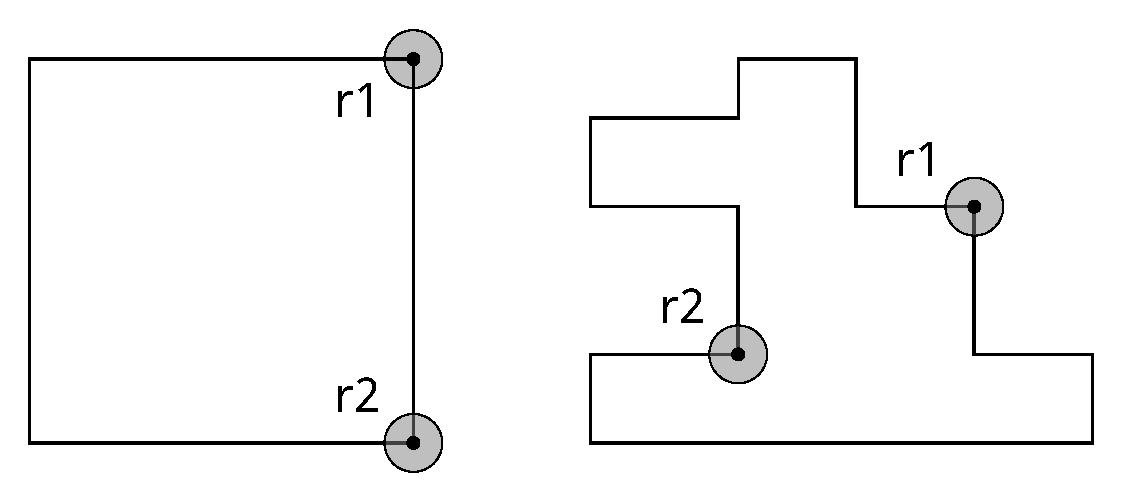
\includegraphics[height=\imgHeight]{images/rsimilarity.pdf}
    \caption{Beispiel für r-Ähnlichkeit.}
    \label{fig:rsimilarity}
\end{figure}

Die hier verwendete lokale Ähnlichkeit funktioniert nach dem gleichen Konzept, mit der Ausnahme, dass der Radius so klein wie möglich gehalten
wird. Wir schauen uns also lediglich an, welche Kanten und Polygone direkt an einem Punkt anliegen, während uns die restliche Nachbarschaft
egal ist. So können die betrachteten Strukturen beliebig skaliert werden und trotzdem ihre lokale Ähnlichkeit zueinander bewahren, solang alle
Kantenwinkel dabei beibehalten werden.

\subsection{Planarität und der Graph Boundary String}
Damit die erzeugten Winkelgraphen später auch ohne Überschneidungen der Kanten dargestellt werden können, muss sichergestellt werden, dass diese
planar sind. Die letztendlich erzeugten vollständigen Winkelgraphen bestehen nur noch aus geschlossenen Kreisen. Diese können dann als Polygone
dargestellt werden, vorausgesetzt der jeweilige Kreis war planar.

Ein geschlossener Kreis ist planar, wenn wir uns beim Traversieren seiner Kanten exakt einmal um 360° gedreht haben. Wenn wir also iterativ
alle Kanten eines solchen Kreises gegen den Uhrzeigersinn betrachten, jeweils die Differenz der Winkel berechnen und diese Differenzen
aufsummieren, so erhalten wir einen Gesamtwinkel von 360°. Es kann allerdings auch vorkommen, dass wir beim Entlanglaufen eines Pfades um
einen geschlossenen Kreis herum einen Gesamtwinkel von mehr als 360° erhalten, so z.B. 720°. Ist dies der Fall, so muss sich der Pfad zwingend
selbst gekreuzt haben. Analog würde es bei der Darstellung der Kanten des entsprechenden Kreises mindestens eine unvermeidliche Überschneidung
geben. Somit wäre der Winkelgraph, der diesen Kreis enthalten hat, nicht mehr planar, was ebenfalls in Abbildung \ref{fig:planarity} zu erkennen ist.

\begin{figure}[t]
    \centering
    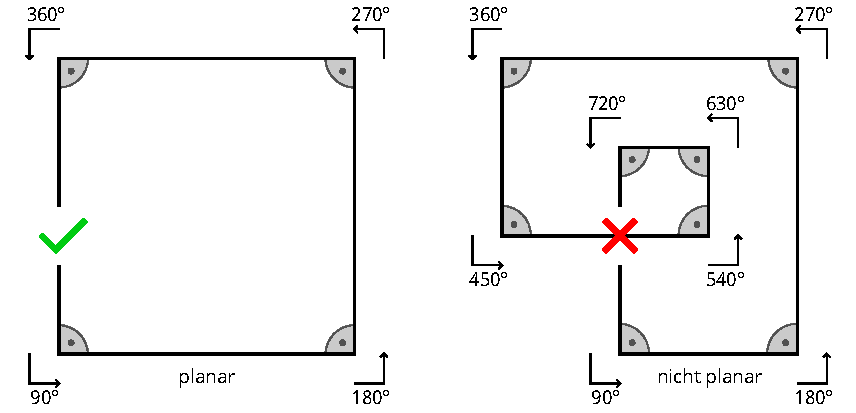
\includegraphics[width=(\imgWidth*3/4)]{images/planarity.pdf}
    \caption{Der Zusammenhang zwischen Drehwinkel und Planarität.}
    \label{fig:planarity}
\end{figure}

Zum Vorbeugen dieses Problems definieren wir hier das Konzept der \textit{Graph Boundary} und die dazugehörige Notation in Form vom
\textit{\gls{ac:gbs}}. Jeder Winkelgraph besitzt eine solche Boundary. Diese beschreibt einen Pfad außen um den entsprechenden
Winkelgraphen herum und enthält alle vorhandenen Halbkanten, sowie Informationen dazu, wie sich die Winkel entlang des Pfades ändern.
Der Pfad verläuft gegen den Uhrzeigersinn und hat keinen festen Startpunkt. Wichtig ist lediglich die relative Anordnung der enthaltenen
Elemente. Um dies abbilden zu können, muss sich der \gls{ac:gbs} nicht als Liste mit festem Start- und Endpunkt vorgestellt werden,
sondern als Kreis mit einer zusätzlichen Verbindung zwischen Anfang und Ende. Angenommen \(abc\wedge\) ist ein \gls{ac:gbs}, dann gilt
\(abc\wedge = bc\wedge a = c\wedge ab = \wedge abc\).

Um den aktuellen Drehwinkel in Relation zum Startpunkt des Pfades zu ermitteln, können wir uns jeweils die Kantenlabel der traversierten
Kanten anschauen und dort den Tangentenwinkel entnehmen. Dies wird allerdings problematisch, sobald sich der Pfad um mehr als
360° dreht, da die Tangentenwinkel bei 180° bzw. -180° umgebrochen werden. Berechnen wir den aktuellen Drehwinkel entlang der Boundary mithilfe
dieser Tangentenwinkel, so können wir nie eine Differenz von über 360° erhalten. Haben wir uns vom Startpunkt aus z.B. tatsächlich um 400°
gedreht, so würde die hier berechnete Differenz lediglich \(400\degree - 360\degree = 40\degree\) betragen. Analog wissen wir nie, ob wir uns
aktuell um den Winkel \(\theta\), \(\theta + 360\degree\), \(\theta + 720\degree\) oder noch mehr gedreht haben.
Dieses Problem lässt sich durch Einführung des Konzepts der \textit{positiven und negativen Drehungen} umgehen.

\textit{Positive Drehung \(\wedge\).} Dreht sich der Pfad aktuell gegen den Uhrzeigersinn wird der Winkel mit jeder gefundenen Kante größer. Stoßen wir
dabei allerdings auf den Schwellwert von 180°, so bricht der Winkel auf einmal in den negativen Bereich um. Diesen Umbruch bezeichnen wir als
positive Drehung. Finden wir also beim Entlanglaufen des Pfades erst eine positiv und dann eine negativ verlaufende Kante, so fügen wir eine
positive Drehung in Form des Symbols \(\wedge\) in den \gls{ac:gbs} ein. Die Boundary eines planaren Winkelgraphen muss zwingend eine
solche positive Drehung enthalten.

\textit{Negative Drehung \(\vee\).} Die negative Drehung stellt das Gegenteil zur positiven Drehung dar. Dreht sich der Pfad aktuell mit dem
Uhrzeigersinn, so nähern sich die gefunden Winkel nach und nach dem Schwellwert von -180°. Anschließend bricht der Winkel in den positiven Bereich
um, was wir als negative Drehung bezeichnen und mit dem Symbol \(\vee\) im \gls{ac:gbs} notieren.

Diese beiden Drehungen heben sich gegenseitig auf. Die Differenz zwischen den positiven und negativen Drehungen in einem Winkelgraphen muss also
exakt 1 betragen, damit dieser planar ist. Befinden sich eine positive und eine negative Drehung nebeneinander im \gls{ac:gbs}, so können
diese entfernt werden. Ebenfalls kann an jeder beliebigen Stelle ein \(\wedge\vee\) oder ein \(\vee\wedge\) eingefügt werden, ohne die Bedeutung
des jeweiligen \gls{ac:gbs} zu verändern.

% TODO: Abbildung von Winkelgraph mit dazugehörigem Boundary String etc.

\subsection{Teil-Operation}
Eine Kante \(\tilde{k}\) kann in zwei Halbkanten \(k\) und \(\overline{k}\) zerteilt werden. Im Gegensatz zu \(\tilde{k}\)
sind diese beiden Halbkanten gerichtet und zeigen in entgegengesetze Richtungen. Dabei zeigt k stets in positive Richtung und besitzt einen
positiven Tangentenwinkel \(\theta \in [0\degree,180\degree) \), während \(\overline{k}\) immer in negative Richtung zeigt und einen negativen
Tangentenwinkel \(\theta \in [-180\degree,0\degree) \) besitzt. Ein Tangentenwinkel von 0° zählt hier als positiv. Der entgegengesetze Winkel
von 180\degree\ gilt als negativ, da dieser ebenfalls als -180\degree\ interpretiert werden kann. Die Teil-Operation ermöglicht das Zerlegen vom
Input in die jeweiligen Primitive.

\subsection{Klebe-Operation}
Zwei entgegengesetze Halbkanten \(k\) und \(\overline{k}\) können wieder zu einer vollständigen und ungerichteten Kante
\(\tilde{k}\) zusammengeklebt werden. Dies ermöglicht das Schließen von Kreisen innerhalb eines Graphen oder die Kombination von mehreren
kleineren Graphen, vorausgesetzt diese besitzen passende Halbkanten. Hier ist erneut der \gls{ac:gbs} von Relevanz, da aus diesem alle
möglichen Klebe-Operationen abgeleitet werden können, welche die Planarität der entstehenden Graphen bewahren. Grundlegend gibt es zwei
verschiedene Arten von Klebe-Operationen: Loop Gluing und Branch Gluing.

\textit{Loop Gluing} beschreibt das Zusammenkleben zweier Kanten innerhalb eines einzigen Graphen. Das Anwenden einer solchen Operation
führt zum Schließen eines Kreises innerhalb des Graphen. Ob ein Loop Gluing auf einen Graphen angewandt werden kann, lässt sich durch das
Vorhandensein eines der zwei Teilstrings \(a \overline{a}\) oder \(\overline{a}\vee a\wedge\) innerhalb des \gls{ac:gbs} ermitteln. Werden
die gefundenen Kanten dann zusammengeklebt, muss der \gls{ac:gbs} noch entsprechend angepasst werden. Für das Loop Gluing ist diese Anpassung
besonders einfach und es muss lediglich der gefundene Teilstring entfernt werden. Die entsprechenden String-Ersetzungen besitzen die Form:

\begin{center}
    \(a \overline{a} \longrightarrow \epsilon\) \ \ \ bzw. \ \ \ \(\overline{a}\vee a\wedge \longrightarrow \epsilon\) 
\end{center}

\textit{Branch Gluing} beschreibt das Zusammenkleben zweier Kanten von verschiedenen Graphen. Dies führt zur Vereinigung der beiden betroffenen
Graphen in einen neuen, größeren Graphen. Besitzt Graph G die Kante \(\overline{a}\) und Graph H die Kante \(a\), so kann ein Branch Gluing
durchgeführt werden. Hierbei gibt es wieder zwei Optionen:

\begin{center}
    \(\overline{a}G\) an \(a\): \(a \longrightarrow G \vee\) \ \ \ bzw. \ \ \ \(a H\) an \(\overline{a}\): \(\overline{a} \longrightarrow \vee H\)
\end{center}

Die Großbuchstaben G und H stehen hier jeweils für den Rest des \gls{ac:gbs}s der Graphen G und H. Der \gls{ac:gbs} des neu enstandenen Graphen
stellt die Kombination der beiden kleineren \gls{ac:gbs}s dar, allerdings ohne die zusammengeklebten Halbkanten und mit einer zusätzlichen
negativen Drehung.

% TODO: Abbildung der Gluing Operationen

\section{Ablauf}
\subsection{Anpassen des Inputs}
Bevor wir mit dem Verfahren beginnen können, muss der Input an bestimmte Anforderungen angepasst werden. Die übergebene Polygonstruktur
kann so nicht direkt verarbeitet werden und muss erst einmal in einen Winkelgraphen umgewandelt werden. Ohne diesen Schritt liegen uns keine
Informationen zu den Kantenwinkeln vor, welche ausschlaggebend für die weiteren Schritte sind. Hierzu werden zunächst einfach alle Knoten und
Kanten aus dem Input übernommen. Anschließend werden die Knotenpositionen genutzt, um den Verlauf der Kanten in Form eines Tangentenwinkels zu
ermitteln. Sobald dies geschehen ist, können die Knotenpositionen dann ignoriert werden, da lediglich die Ausrichtung der Kanten eine Rolle
für die weiteren Schritte spielt. Die restlichen Informationen zur Geometrie werden nicht benötigt und erst beim Erzeugen des finalen Outputs
wieder festgelegt.

\subsection{Finden der Primitive}
Ist nun der Winkelgraph ermittelt worden, können wir daraus die Primitive ableiten. Diese sind die fundamentalen Grundbausteine für das
gesamte Verfahren. Aus ihnen werden alle weiteren Strukturen abgeleitet, weshalb es besonders wichtig ist, diese korrekt und vollständig zu
ermitteln. Glücklicherweise wird dies durch die vorgestellte Teil-Operation recht trivial. Wenden wir diese auf jede Kante des gegebenen
Winkelgraphen an, so bleiben nur Teilgraphen übrig, welche nur aus einem einzelnen Knoten, sowie einigen Halbkanten bestehen. Diese Teilgraphen
sind dann auch schon die gesuchten Primitive. Hier können allerdings einige identische Teilgraphen entstehen, falls Teile des Input eine ähnliche
Struktur vorzuweisen hatten. Solche Duplikate sind natürlich nicht relevant für die weiteren Schritte und werden ignoriert.

\subsection{Aufbauen der Graph-Hierarchie}
Die vorgestellten Klebe-Operationen ermöglichen es uns, die gefundenen Primitive nach und nach zu komplexeren Graphen zusammenzusetzen.
Diese lassen sich in verschiedene Generationen einer Hierarchie einordnen. In Generation 0 befinden sich alle verschiedenartigen
Kanten, also alle Kanten mit einem einzigartigen Kantenlabel. In Generation 1 befinden sich alle gefundenen Primitive. Anschließend können
die nachfolgenden Generationen automatisch generiert werden. Dazu werden alle Winkelgraphen der zuletzt generierten Generation enumeriert
und alle möglichen Klebe-Operationen angewandt. Zu den möglichen Klebe-Operationen zählen zum einen das Schließen von Kreisen innerhalb einzelner
Graphen durch Loop Gluing, und zum anderen alle Branch Gluing Operationen zwischen den enumerierten Graphen und den gefundenen Primitives.
Wird eine mögliche Klebe-Operation gefunden und dadurch ein neuer Graph erzeugt, so gilt dieser als Kind des anderen Graphen. Jeder Graph wird
also neben der Einordnung in eine Generation außerdem in eine Eltern-Kind-Beziehung gebracht. Die Struktur der Hierarchie selbst ähnelt somit
fast der eines Baumes, allerdings kann ein und derselbe Kindsgraph durch verschiedene Elterngraphen erzeugt werden, wodurch wiederum Kreise
innerhalb der Hierarchie entstehen.

In der Theorie können alle Kombinationen an Primitiven erzeugt werden, wenn wir dieses Vorgehen bis in die Unendlichkeit weiterführen. Somit
würden garantiert alle zum Input lokal ähnlichen Winkelgraphen erzeugt werden und man könnte einfach jeden beliebigen vollständigen Graphen
aus der Hierarchie entnehmen, um jeden validen Output des Verfahrens erzeugen zu können. Praktisch gesehen ist dies natürlich leider nicht
umsetzbar, da uns weder unendlich viele Ressourcen noch Zeit zur Verfügung stehen. Um diesen Ansatz also praktisch zu machen, müssen einige
Anpassungen gemacht werden.

\subsection{Ableiten der Graph-Grammatik}
Statt zuerst eine ``vollständige'' Hierarchie zu erzeugen und aus
dieser dann weitere Schritte abzuleiten, wird die Hierarchie inkrementell erzeugt. Jedes Mal, wenn ein neuer Graph erstellt wird, überprüfen
wir diesen auf bestimmte Eigenschaften, die es uns erlauben daraus Regeln für eine Graph-Grammatik abzuleiten. Ein solche Regel ermöglicht es
uns bereits erzeugte Winkelgraphen zu reduzieren, was wiederum bedeutet, dass wir diese nicht mehr benötigen und aus der Hierarchie entfernen
können. Ein detaillierter Einblick zu der Theorie dahinter wird erst in den folgenden Unterkapiteln gegeben, jedoch ist es genau diese Eigenschaft,
die es uns ermöglicht, das Wachstum der Hierarchie einzugrenzen. Optimalerweise erreichen wir irgendwann einen Punkt, an dem alle bereits erzeugten
Graphen durch eine der Regeln reduziert werden konnten. In diesem Fall können wir garantieren, dass sich aus den Regeln alle vollständigen
und zum Inputgraphen lokal ähnlichen Winkelgraphen aus der erzeugten Grammatik ableiten lassen. Meistens werden wir allerdings auf
Szenarien stoßen, in denen die Anzahl der neuen Graphen schneller wächst, als wir andere Graphen entfernen können. Kommt dies vor, so muss das
Erstellen der Hierarchie irgendwann frühzeitig abgebrochen werden und die Graph-Grammatik ist eventuell nicht in der Lage, alle lokal ähnlichen
Graphen zu erzeugen. Trotzdem kann die Grammatik dann zum Ableiten einer Vielzahl von lokal ähnlichen Winkelgraphen genutzt werden.

\subsubsection{Graph-Grammatiken}
Bevor wir die Erzeugung dieser Datenstruktur genauer betrachten, soll erst einmal der Begriff der Graph-Grammatik klar definiert werden.
Eine Graph-Grammatik ist ein formales System, welches spezifisch auf die Erstellung und Manipulation von Graphen in einem mathematisch
präzisen Weg abzielt. Dazu wird eine Menge an Produktionsregeln definiert, welche verschiedene Operationen zum Ersetzen von Teilen
eines Graphen beschreiben. Eine solche Produktion besteht üblicherweise aus drei Bestandteilen: zwei Graphen \(M\) und \(T\) (``Mutter'' und
``Tochter''), sowie einem Einbettungsmechanismus \(E\). Diese Produktion kann nun auf jeden Graphen \(G\) angewandt werden, welcher \(M\)
als Teilgraphen enthält. Um die Produktion anzuwenden, wird \(M\) aus \(G\) entfernt und mit \(T\) ersetzt. Dabei wird \(E\) genutzt, um zu
definieren, wie genau \(T\) in \(G\) eingebettet werden kann. \cite{31_engelfriet_rozenberg}

Das Konzept der Graph-Grammatiken existiert bereits seit den frühen 70er Jahren und wurde mit dem Paper von Ehrig et al. \cite{7_ehrig_et_al}
zum ersten Mal formal definiert. Seitdem haben sich sehr viele verschiedene Herangehensweisen in diesem Kontext etabliert, was zu viel Verwirrung
führen kann. \cite{30_könig_et_al} Wir beschränken uns hier auf den ursprünglich präsentierten algebraischen bzw. Gluing-Ansatz von Ehrig 
et al. \cite{7_ehrig_et_al}. Innerhalb dieses Ansatzes haben sich zwei verschiedene Vorgehensweisen etabliert: der Single Pushout Ansatz und der
\gls{ac:dpo} Ansatz, wovon wir den letzteren verwenden. Der Begriff ``Pushout'' stammt aus der Kategorientheorie, welche ebenfalls zum Beschreiben
von Graph-Grammatiken genutzt werden kann. \cite{1_merrell}

\begin{figure}[t]
    \centering
    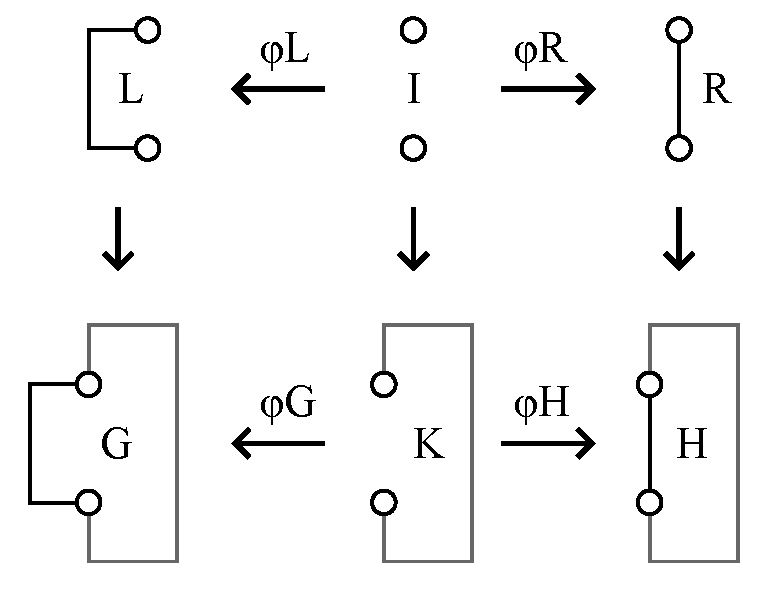
\includegraphics[width=\imgWidth/2]{images/dpo_rule.pdf}
    \caption{Double Pushout Produktionsregel.}
    \label{fig:dpo_rule}
\end{figure}

Die Produktionen im verwendeten \gls{ac:dpo} Ansatz bestehen aus drei Teilen. Einem linken und rechten Graphen (\(L\) und \(R\)), welche jeweils
den Mutter- und Tochtergraphen darstellen, sowie einem Interface-Graphen \(I\), welcher den Einbettungsmechanismus darstellt.Wie in Abbildung
\ref{fig:dpo_rule} zu sehen ist, können diese Graphen mithilfe der Graphmorphismen \(\upvarphi L\) und \(\upvarphi R\) untereinander abbilden.
Ist \(L\) als Teilgraph in einem anderen Graphen \(G\) enthalten, so kann die entsprechende Produktion zum Transformieren von \(G\) verwendet werden.
Dazu muss \(L\) zunächst aus \(G\) herausgeschnitten werden. Hierfür wird das Interface benötigt. Dieses beschreibt die Gemeinsamkeiten zwischen
der linken und der rechten Seite der Produktion und ermöglicht das problemlose Austauschen der beiden Seiten miteinander. Wird \(L\) aus \(G\)
entfernt, so erhalten wir den sogenannten Klebegraphen \(K\). In diesen können wir nun \(R\) hineinkleben, um den transformierten Graphen \(H\)
zu erhalten. Das Anwenden einer solchen Produktionsregel ist aber auch in die andere Richtung möglich. Alternativ kann auch zuerst \(R\) aus
\(H\) ausgeschnitten und dann dort \(L\) eingeklebt werden, um \(G\) zu produzieren. \cite{7_ehrig_et_al}

\subsubsection{Theorie hinter der Funktionsweise}
Die später aus der Hierarchie abzuleitenden Produktionsregeln werden so angeordnet, dass sich auf der linken Seite ein komplexerer Graph befindet,
als auf der rechten Seiten. Wird die Regel von links nach rechts angwendet, so vereinfacht sie \(G\). Dies bezeichnen wir als \textit{destruktiv}.
Wird sie von rechts nach links angewendet, so macht sie \(H\) komplexer, was wir wiederum als \textit{konstruktiv} berzeichnen. \cite{1_merrell}

Wie bereits erwähnt, versuchen wir nach dem Erstellen der einzelnen Graphen Regeln zu finden, die bereits erzeugte Graphen in der Hierarchie
vereinfachen können und entfernen diese dann ggf. aus der Hierarchie. Hier werden die Regeln stets nur destruktiv genutzt, was zunächst unlogisch
erscheint. An diesem Punkt können wir uns die Invertierbarkeit der Produktionen zunutze machen. Wenn wir genug Regeln finden können, um alle Graphen
in der Hierarchie zum leeren Graphen reduzieren zu können, indem wir diese destruktiv verwenden, so können wir im Umkehrschluss genau die gleichen
Regeln konstruktiv benutzen, um aus dem leeren Graphen alle anderen Graphen abzuleiten. \cite{1_merrell}

%\subsubsection{Ableiten einer Produktionsregel}
% Zuerst eingehen auf Zusammenhang mit dem GBS (Merrell 5.0)

%\subsubsection{Sonderfälle bei der Bildung von Produktionsregeln}

% TODO:
% - Erstellen von Abbildungen: 1/3
% - Hinzufügen von Quellen

% @author Benjamin Schröder
%
\chapter{Implementation}
% @author Benjamin Schröder
%
\chapter{Auswertung}
% @author Benjamin Schröder
%
\chapter{Fazit}

%\bibliographystyle{plain}
\bibliographystyle{dinat}
\bibliography{literature}

% Appendix
\appendix
% !TEX root = ../thesis.tex
% appendix example chapter
% @author Thomas Lehmann
%

\chapter{Anhang}

\section{Verwendete Hilfsmittel}
In der Tabelle \ref{tab:tooling} sind die im Rahmen der Bearbeitung des Themas der \IthesisKindDE~verwendeten Werkzeuge und Hilfsmittel aufgelistet.

\begin{table}[h!]
\caption{Verwendete Hilfsmittel und Werkzeuge}
\begin{tabular}{|l|l|}
\hline 
\rowcolor{lightgray} Tool & Verwendung \\
\hline
\LaTeX & Textsatz- und Layout-Werkzeug verwendet zur Erstellung dieses Dokuments \\
\hline
 & \\
\hline
\end{tabular}
\label{tab:tooling}
\end{table}



\IGlossary

\Istatement

\end{document}

% compile using the following commands:
%
% pdflatex thesis.tex
% bibtex thesis
% makeglossaries thesis
% pdflatex thesis.tex
% pdflatex thesis.tex
